\documentclass[a4paper,11pt]{article}
\usepackage[french]{babel}
\usepackage[margin=2.5cm]{geometry}
\usepackage{lipsum}
\usepackage{amsmath}
\usepackage{amssymb}

\usepackage{tikz}
\usetikzlibrary{arrows.meta, positioning}

\usepackage{graphicx}
\graphicspath{{figures/}{../../results/}}

\usepackage{booktabs}
\usepackage{array}
\usepackage{caption}
\usepackage{subcaption}
\usepackage{float}
\usepackage{xcolor}

\usepackage{lmodern}
\usepackage[autostyle=true]{csquotes}

\usepackage[backend=biber,style=ieee]{biblatex}
\addbibresource{references.bib}
%%% Use the package for UMONS cover page
% the option describe the faculty you belong to
% e.g. fpms, fs, ...
\usepackage[fpms]{umons-coverpage}
\umonsAuthor{Canfyn \textsc{Marie} \newline Drogo \textsc{Flavio}\newline Groupe 05 }
% The main title of your thesis
\umonsTitle{Machine and Deep Learning for Multimedia Retrieval}
% The sub-title of your thesis
\umonsSubtitle{I-ILIA-014}
% The type of document: the reason of the thesis
\umonsDocumentType{Rapport de projet \newline
                    Quadrimestre 2
                    } 
% Grades possibles : Master Ingénieur Civil Architecte, Master Ingénieur Civil en Chimie et Science des Matériaux, Master Ingénieur Civil Electricien, Master Ingénieur Civil en Informatique et Gestion, Master Ingénieur Civil Mécanicien, Master Ingénieur Civil en Mines et Géologue
% Your supervisor(s)
%\umonsSupervisor{Sous la direction de  : \\
%Madame/Monsieur Professeur Prenom \textsc{Nom} (promoteur)\\
%Madame/Monsieur Prenom \textsc{Nom} (co-promoteur) \\
%Madame/Monsieur Prenom \textsc{Nom} (rapporteur)} 
% The date (or academic year)
\umonsDate{Année académique 2026-2026}

\begin{document}

% Ask for a regular cover page with full content and default picture
\umonsCoverPage

\pagenumbering{gobble}
\tableofcontents
\newpage

\pagenumbering{arabic}
\setcounter{page}{1}

\section{Introduction}

\subsection{Contexte et motivation}

La croissance exponentielle des contenus multimédias disponibles en ligne (images, vidéos, textes) a fait de la recherche d'information multimédia (\textit{Multimedia Information Retrieval}, MIR) un domaine central de l'intelligence artificielle moderne. Qu'il s'agisse de retrouver une photographie dans une collection personnelle, d'identifier un produit à partir d'une image, ou encore d'interroger une base de données à l'aide d'une description textuelle, les moteurs de recherche multimédias sont devenus des outils incontournables. Leur efficacité repose sur la qualité des descripteurs utilisés pour représenter le contenu, ainsi que sur les mesures de similarité employées pour comparer ces représentations.

Historiquement, les approches classiques s'appuyaient sur des descripteurs \textit{hand-crafted} tels que les histogrammes de couleurs, SIFT ou HOG. L'avènement de l'apprentissage profond a profondément transformé le domaine en permettant l'extraction automatique de caractéristiques sémantiquement riches via des réseaux de neurones convolutifs (CNN) et, plus récemment, via des architectures de type \textit{Vision Transformer} (ViT). Par ailleurs, des modèles multimodaux comme CLIP~\cite{radford2021learningtransferablevisualmodels} ont ouvert la voie à une recherche véritablement \textit{cross-modale}, où l'image et le texte partagent un même espace de représentation.

\subsection{Objectifs du projet}

Ce projet, réalisé dans le cadre du cours \textit{Machine and Deep Learning for Multimedia Retrieval}, a pour but de concevoir, implémenter et déployer une application complète de recherche multimédia. Il s'articule autour de trois parties complémentaires~:

\begin{itemize}
    \item \textbf{Partie I - Moteur de recherche unimodal~:} développement d'un moteur d'indexation et de recherche d'images sur la base \textit{Cars} (10\,000 images réparties en 10 marques et 96 marques+modèles), à partir de descripteurs variés incluant au moins un descripteur CNN et un descripteur ViT. Plusieurs mesures de similarité sont comparées, et les performances sont évaluées à l'aide des métriques usuelles (Precision, Recall, AP, mAP, R-Precision).

    \item \textbf{Partie II - Moteur de recherche multimodal~:}
    mise en place d'un moteur \textit{text-to-image} et \textit{image-to-text} sur la base \textit{Flickr8K}, en exploitant le modèle CLIP pour projeter les images et les textes dans un espace latent commun. L'indexation repose sur FAISS afin d'assurer une recherche efficace des plus proches voisins. Un second modèle contrastif (BLIP/OpenCLIP) est également évalué à titre comparatif.

    \item \textbf{Partie III - Déploiement cloud~:}
    encapsulation de l'application dans une image Docker et mise à disposition via une interface web Flask sous forme de service SaaS. Cette partie inclut également une réduction de la dimensionnalité des descripteurs ainsi qu'une analyse de la sécurité du site.
\end{itemize}

\subsection{Organisation du rapport}

La suite du rapport est organisée comme suit. La Section~\ref{sec:part1} présente le moteur de recherche unimodal, les descripteurs utilisés et les résultats expérimentaux obtenus sur la base \textit{Cars}. La Section~\ref{sec:part2} détaille l'approche multimodale fondée sur CLIP et son évaluation sur \textit{Flickr8K}. La Section~\ref{sec:part3} décrit le déploiement de l'application dans un environnement cloud, incluant l'interface web, la réduction de dimensionnalité et les aspects de cybersécurité. Enfin, la Section~\ref{sec:conclusion} conclut le rapport et propose quelques pistes d'amélioration.

\newpage
\section{Moteur de recherche d'images uni modal à deux niveaux}
\label{sec:part1}

\subsection{Position du problème}

Étant donné un corpus d'images $\mathcal{D} = \{I_1, I_2, \dots, I_N\}$ 
réparties en $C$ classes sémantiques, le problème de la recherche d'images 
par le contenu (\textit{Content-Based Image Retrieval}, CBIR) peut être 
formulé de la manière suivante~: comment construire une fonction 
$\varphi : \mathcal{I} \rightarrow \mathbb{R}^d$, appelée \emph{descripteur} 
ou \emph{extracteur de caractéristiques}, qui projette chaque image dans un 
espace latent de dimension $d$, de telle sorte que les images 
sémantiquement proches soient également proches au sens d'une certaine 
mesure de similarité $s(\cdot, \cdot)$~?

Formellement, on cherche $\varphi$ telle que, pour toute image requête 
$I_q$ et toute image $I_j$ du corpus~:
\begin{equation}
    \text{classe}(I_q) = \text{classe}(I_j) 
    \;\Longrightarrow\; 
    s\bigl(\varphi(I_q), \varphi(I_j)\bigr) \text{ est élevée},
    \label{eq:cbir_objective}
\end{equation}
tandis que les images de classes différentes doivent être éloignées dans 
cet espace latent. Autrement dit, une "bonne" transformation $\varphi$ 
est celle qui maximise la compacité intra-classe et la séparation 
inter-classe des descripteurs, un objectif proche de celui du 
\textit{metric learning}.

Une fois ce plongement défini, la recherche se ramène à un problème de 
plus proches voisins~: pour une image requête $I_q$, on calcule 
$\varphi(I_q)$, puis on retourne les $k$ éléments du corpus dont les 
descripteurs minimisent une distance choisie (euclidienne, cosinus, 
$\chi^2$, Bhattacharyya, etc.).

\subsection{Approches envisagées}

Le choix de la transformation $\varphi$ est donc \emph{la} question 
centrale de cette partie. Historiquement, deux grandes familles 
d'approches coexistent~:

\begin{itemize}
    \item les descripteurs \textbf{classiques} (\textit{hand-crafted}), 
    comme les histogrammes de couleurs, GLCM, HOG ou 
    SIFT, qui reposent sur une modélisation explicite de propriétés 
    visuelles bas-niveau~;
    \item les descripteurs \textbf{profonds}, obtenus en extrayant les 
    activations d'une couche intermédiaire ou finale d'un réseau de 
    neurones pré-entraîné sur une tâche de classification à grande échelle 
    (typiquement ImageNet). On distingue ici les architectures 
    convolutives (CNN) comme ResNet, et les 
    architectures de type \textit{Vision Transformer} 
    (ViT).
\end{itemize}

Conformément à l'énoncé, notre projet comparera plusieurs descripteurs de 
ces deux familles, dont au moins un CNN et un ViT, afin de déterminer 
expérimentalement lequel offre la meilleure séparation des classes de la 
base \textit{Cars}. La Figure~\ref{fig:cbir_pipeline} illustre le pipeline 
global de notre moteur de recherche~: indexation hors-ligne du corpus, 
puis recherche en ligne par comparaison dans l'espace latent.

\begin{figure}[h]
    \centering
    \begin{tikzpicture}[
    font=\small,
    node distance=0.9cm and 1.1cm,
    box/.style={draw, rounded corners, minimum height=0.9cm, 
                minimum width=1.8cm, align=center, fill=blue!8},
    phi/.style={draw, circle, minimum size=0.9cm, fill=orange!25, 
                font=\footnotesize},
    index/.style={draw, rounded corners, minimum height=1.1cm, 
                  minimum width=2.2cm, align=center, fill=green!12},
    arrow/.style={-{Latex[length=2mm]}, thick},
    dashedarrow/.style={-{Latex[length=2mm]}, thick, dashed}
]

% --- Offline branch ---
\node[box] (corpus) {Corpus\\$\{I_1,\dots,I_N\}$};
\node[phi, right=of corpus] (phi1) {$\varphi$};
\node[box, right=of phi1] (desc) {Descripteurs\\$\varphi(I_i)\in\mathbb{R}^d$};
\node[index, right=of desc] (idx) {Index\\(FAISS, kNN)};

\draw[arrow] (corpus) -- (phi1);
\draw[arrow] (phi1) -- (desc);
\draw[arrow] (desc) -- (idx);

% --- Online branch ---
\node[box, below=1.4cm of corpus, fill=red!8] (query) {Requête\\$I_q$};
\node[phi, right=of query] (phi2) {$\varphi$};
\node[box, right=of phi2, fill=red!8] (qdesc) {$\varphi(I_q)$};

\draw[arrow] (query) -- (phi2);
\draw[arrow] (phi2) -- (qdesc);

% --- Similarity search ---
\node[box, right=1.4cm of qdesc, fill=yellow!20] (sim) 
     {Recherche\\$s(\varphi(I_q),\varphi(I_j))$};
\node[box, right=of sim] (topk) {Top-$k$\\images};

\draw[arrow] (qdesc) -- (sim);
\draw[dashedarrow] (idx) -- (sim);
\draw[arrow] (sim) -- (topk);

% --- Labels hors-ligne / en ligne ---
% \node[anchor=west, font=\footnotesize\itshape] 
%      at ([xshift=-1.2cm]corpus.west) {Hors-ligne};
% \node[anchor=west, font=\footnotesize\itshape] 
%      at ([xshift=-1.2cm]query.west) {En ligne};

\end{tikzpicture}
    \caption{Pipeline du moteur de recherche unimodal.}
    \label{fig:cbir_pipeline}
\end{figure}

\subsection{Protocole expérimental}
\label{subsec:protocole}

\paragraph{Base de données \textit{Cars}.}
Le corpus utilisé est composé de $10\,000$ images de véhicules réparties
en $10$ marques (\textit{niveau 1}) et $96$ couples
\textit{marque + modèle} (\textit{niveau 2}). C'est cette double
granularité qui justifie le qualificatif \emph{à deux niveaux} de notre
moteur~: une même requête peut être évaluée à un niveau \emph{grossier}
(retrouver des images de la même marque) ou \emph{fin} (retrouver le même
modèle exact). Conformément à la consigne, nous adoptons systématiquement
la granularité fine~: une image récupérée n'est considérée pertinente que
si elle partage à la fois la marque \emph{et} le modèle de la requête.
Cette définition stricte induit naturellement la pertinence au niveau 1,
puisqu'un même couple marque/modèle implique une marque commune.

\paragraph{Requêtes.}
Conformément au protocole imposé pour le groupe~05, $15$ images réparties
sur $5$ marques ($\{0,2,4,6,8\}$, soit BMW, Volkswagen, Opel, Hyundai et
Ford), à raison de $3$ modèles par marque, sont extraites du corpus pour
servir de requêtes notées $R_1$ à $R_{15}$. Ces images sont \emph{exclues}
de la galerie d'indexation afin d'éviter tout biais d'auto-récupération.
Le nombre d'images pertinentes par classe varie de $42$ à $162$, ce qui
empêche d'atteindre une recall parfaite avec $k\le 100$ et impose donc une
attention particulière aux métriques tronquées.

\paragraph{Distribution intra-classe.}
L'analyse exploratoire (notebook \texttt{00\_data\_analysis}) révèle une
forte variabilité intra-classe~: angles de prise de vue, couleurs,
arrière-plans et éclairages diffèrent largement pour un même modèle. Ce
constat justifie a priori la nécessité de descripteurs sémantiques de
haut niveau plutôt que de simples descripteurs bas-niveau (couleur,
texture).

\subsection{Descripteurs classiques}
\label{subsec:classical}

Trois descripteurs \textit{hand-crafted} couvrant deux familles
complémentaires ont été retenus~:
\begin{itemize}
    \item \textbf{HOG}~(\textit{Histogram of Oriented Gradients}) -
    descripteur \emph{global} de forme. Les images sont converties en
    niveaux de gris, redimensionnées à $256\times 256$ puis encodées par
    un histogramme d'orientations de gradient calculé sur des cellules
    $16\times 16$ regroupées en blocs $2\times 2$ (normalisation
    L2-Hys, $9$ orientations). Le descripteur final est un vecteur dense
    de $\sim 7\,000$ dimensions.

    \item \textbf{SIFT}~(\textit{Scale-Invariant Feature Transform}) et
    \textbf{ORB}~(\textit{Oriented FAST and Rotated BRIEF}) - descripteurs
    \emph{locaux} basés points-clés. Pour produire un vecteur de taille
    fixe et indexable, nous adoptons l'approche \textit{Bag of Visual
    Words}~(BoVW)~: un vocabulaire de $K=256$ mots visuels est appris par
    \texttt{MiniBatchKMeans} sur un échantillon de $200\,000$ descripteurs
    issus de la galerie, puis chaque image est encodée par l'histogramme
    L1-normalisé des occurrences des mots. ORB produit des descripteurs
    binaires sur $32$ octets, tandis que SIFT produit des descripteurs
    flottants de dimension $128$~; tous deux sont projetés dans le même
    espace BoVW de dimension $K$.
\end{itemize}

Les descripteurs de couleur (histogrammes RGB/HSV) et de texture pure
(GLCM, LBP) ont été écartés~: la couleur d'une voiture n'est pas
discriminante au niveau marque/modèle (un modèle existe en plusieurs
teintes) et la texture du véhicule est dominée par celle de
l'arrière-plan, source de bruit.

\subsection{Descripteurs profonds}
\label{subsec:dl}

Conformément à l'énoncé, nous comparons \emph{au moins} un descripteur
CNN et un descripteur ViT. Pour rendre la comparaison équitable, les deux
backbones sont entraînés selon \emph{deux paradigmes} sur le même
\textit{split} train/val ($80/20$, stratifié sur les $96$ classes)~:

\begin{enumerate}
    \item \textbf{Mode \textit{classifier}}~: l'extracteur est suivi d'une
    couche de classification linéaire à $96$ sorties, entraînée par
    descente de gradient sur la perte \texttt{CrossEntropy} avec
    \textit{label smoothing} ($\varepsilon = 0.1$). À l'inférence, la
    tête de classification est retirée et le descripteur retenu est la
    sortie de la couche d'embedding $L_2$-normalisée.

    \item \textbf{Mode \textit{metric learning}}~: la même architecture
    est entraînée directement à structurer l'espace latent par la perte
    \texttt{SubCenter-ArcFace} ($k=3$ sous-centres par classe, marge
    angulaire $m=28.6^{\circ}$, échelle $s=64$), couplée à un sampler
    \texttt{MPerClassSampler} ($m=4$ images par classe et par batch).
\end{enumerate}

\paragraph{Architectures.}
\begin{itemize}
    \item \textbf{CNN}~: \texttt{ConvNeXt-Base} pré-entraîné sur
    ImageNet-22k puis \textit{fine-tuned} sur ImageNet-1k
    (\texttt{convnext\_base.fb\_in22k\_ft\_in1k}). Le \textit{global
    pooling} natif est remplacé par un \textbf{GeM pooling}
    ($p=3$, appris) plus adapté à la recherche fine, suivi d'une
    \textit{batch norm} et d'une couche linéaire de projection vers la
    dimension cible. Images d'entrée~: $384\times 384$.

    \item \textbf{ViT}~: \texttt{DINOv2 ViT-B/14}
    (\texttt{vit\_base\_patch14\_dinov2.lvd142m}), self-supervisé sur
    LVD-142M. Le token \texttt{[CLS]} est utilisé comme représentation
    globale, suivi d'une \textit{batch norm} et d'une couche linéaire
    vers la dimension cible. Images d'entrée~: $224\times 224$.
\end{itemize}

Pour chaque (backbone, mode), nous entraînons cinq variantes à dimension
d'embedding $d \in \{128, 256, 512, 1024, 2048\}$ afin d'étudier le
\emph{compromis taille/performance}. Au moment de l'évaluation, le
descripteur final est obtenu par \textit{Test-Time Augmentation}
(moyennage normalisé entre l'image et son miroir horizontal), pratique
standard en CBIR. Les hyperparamètres principaux sont résumés dans la
Table~\ref{tab:hyperparams_dl}.

\begin{table}[H]
\centering
\small
\begin{tabular}{lcccc}
\toprule
Backbone & Img.~size & Optim.~ & LR (\textit{clf} / \textit{metric}) & Epochs (\textit{clf} / \textit{metric}) \\
\midrule
ConvNeXt-Base    & $384$ & AdamW & $3{\cdot}10^{-4}$ / $1{\cdot}10^{-4}$ & $15$ / $20$ \\
DINOv2 ViT-B/14  & $224$ & AdamW & $2{\cdot}10^{-4}$ / $5{\cdot}10^{-5}$ & $15$ / $20$ \\
\bottomrule
\end{tabular}
\caption{Hyperparamètres d'entraînement des descripteurs profonds. Les
deux modes utilisent un \textit{cosine scheduler} avec $2$ epochs de
\textit{warm-up} et un \textit{weight decay} de $10^{-4}$.}
\label{tab:hyperparams_dl}
\end{table}

\subsection{Mesures de similarité et fusion}
\label{subsec:metrics}

Conformément à la consigne, qui mentionne explicitement \emph{Euclidean
distance, Correlation, Chi-square, Bhattacharyya, Brute Force Matcher,
FLANN}, le moteur supporte deux familles de comparaison.

\paragraph{Distances vectorielles.}
Pour les descripteurs déjà agrégés en vecteurs de taille fixe (HOG,
BoVW, embeddings profonds), quatre mesures sont disponibles~:
\begin{align*}
d_{\text{Euc}}(\mathbf{u},\mathbf{v}) &= \lVert \mathbf{u}-\mathbf{v}\rVert_2,
&
d_{\text{corr}}(\mathbf{u},\mathbf{v}) &= 1 - \frac{\mathbf{u}^{\top}\mathbf{v}}{\lVert\mathbf{u}\rVert_2\,\lVert\mathbf{v}\rVert_2}, \\[2pt]
d_{\chi^2}(\mathbf{u},\mathbf{v}) &= \tfrac{1}{2}\sum_i \frac{(u_i-v_i)^2}{u_i+v_i+\varepsilon},
&
d_{\text{Bhatt}}(\mathbf{u},\mathbf{v}) &= -\ln\!\left(\sum_i \sqrt{\hat u_i \hat v_i}\right),
\end{align*}
où $\hat{\mathbf u}$ désigne la version normalisée à somme unitaire de
$\mathbf u$. $d_{\text{corr}}$ correspond à la \emph{distance de
corrélation} (1 moins la similarité cosinus) attendue par l'énoncé~; sur
des descripteurs déjà $L_2$-normalisés, elle est rigoureusement
équivalente à la distance euclidienne au carré, à un facteur près. Les
divergences $\chi^2$ et de Bhattacharyya sont quant à elles spécialement
conçues pour comparer des \emph{distributions} et conviennent donc bien
aux histogrammes BoVW de SIFT et ORB.

\paragraph{Matching de points-clés.}
Pour les baselines SIFT et ORB sans agrégation BoVW (notebook
\texttt{01\_descriptor\_tests\_classique}), les images sont comparées
\emph{point-à-point}~:
\begin{itemize}
    \item \textbf{FLANN-based matcher} (KDTree, $5$ arbres,
    \texttt{checks=50}) pour les descripteurs SIFT (flottants,
    dim.~$128$), avec le \textit{ratio test} de Lowe ($0.7$) pour ne
    conserver que les correspondances fiables~;
    \item \textbf{Brute Force Matcher} (\texttt{cv2.BFMatcher},
    \texttt{NORM\_HAMMING}) pour les descripteurs binaires ORB,
    également filtré par \textit{ratio test} ($0.75$).
\end{itemize}
Les images de la galerie sont alors triées par nombre de bons matchs
décroissants. Cette approche est utilisée à des fins comparatives mais
n'est pas retenue pour le moteur final, le coût quadratique du matching
étant prohibitif (cf. Section~\ref{subsec:results_part1}).

\paragraph{Recherche multi-descripteurs (fusion par rang).}
Pour exploiter la complémentarité éventuelle des descripteurs, le moteur
permet de combiner plusieurs représentations via une fusion
\textit{Reciprocal Rank Fusion} (RRF)~:
\begin{equation}
    \mathrm{score}_{\text{RRF}}(I_j) = \sum_{\varphi \in \mathcal{F}} \frac{1}{c + \mathrm{rang}_\varphi(I_j)},
    \qquad c = 60,
    \label{eq:rrf}
\end{equation}
où $\mathcal{F}$ est l'ensemble des descripteurs sélectionnés et
$\mathrm{rang}_\varphi(I_j)$ est la position de l'image $I_j$ dans le
classement induit par $\varphi$. Cette fusion non paramétrique évite
toute calibration des distances entre descripteurs hétérogènes et a été
retenue pour sa robustesse en pratique. Lorsque $|\mathcal{F}|=1$, on
retombe sur la recherche mono-descripteur.

\subsection{Métriques d'évaluation}
\label{subsec:eval_metrics}

L'évaluation suit les recommandations classiques en CBIR. Pour une
requête $I_q$ de classe $c_q$ et un classement tronqué au rang $k$, on
définit~:
\begin{align}
    P@k &= \frac{1}{k}\sum_{i=1}^{k} \mathbb{1}[c_{r_i}=c_q], &
    R@k &= \frac{1}{n_{c_q}}\sum_{i=1}^{k} \mathbb{1}[c_{r_i}=c_q], \\
    AP@k &= \frac{1}{\min(k, n_{c_q})}\sum_{i=1}^{k} \mathbb{1}[c_{r_i}=c_q]\,P@i,
\end{align}
où $r_i$ est la $i$-ème image renvoyée et $n_{c_q}$ le nombre total
d'images pertinentes dans la galerie. Le \emph{mean Average Precision}
$\text{mAP}@k$ est la moyenne de $AP@k$ sur les $15$ requêtes. Nous
rapportons aussi la \textbf{R-Precision}, définie comme $P@n_{c_q}$~:
elle est moins sensible au choix arbitraire de $k$ et reflète mieux la
qualité globale du classement quand $n_{c_q}$ varie fortement entre
classes (ce qui est notre cas, $n_{c_q} \in [42,\,162]$).

\paragraph{Choix des $k$.}
L'énoncé impose deux $k$ différents pour deux finalités~:
\begin{itemize}
    \item l'\emph{affichage} des images retournées (étape~3) doit se
    faire en \textbf{Top-20} et \textbf{Top-50}~; ces deux profondeurs
    sont disponibles dans l'interface web (Section~\ref{sec:part3}) via
    un slider \emph{Top-K}~;
    \item le \emph{calcul des métriques} (étape~4 et Table~4 de
    l'énoncé) se fait à $k=50$ et $k=100$, ce que nous suivons dans la
    suite.
\end{itemize}

\subsection{Résultats expérimentaux}
\label{subsec:results_part1}

\paragraph{Descripteurs classiques.}
La Table~\ref{tab:classical_results} présente les performances mesurées
sur les $15$ requêtes pour HOG, SIFT et ORB. Les trois descripteurs
peinent à dépasser les $5\%$ de $\text{mAP}@50$, niveau à peine supérieur
à un classement aléatoire compte tenu du déséquilibre des classes. HOG,
purement basé sur les gradients, est dominé par les contours du fond et
reste presque aveugle au contenu sémantique~; ORB et SIFT s'en sortent
légèrement mieux grâce à la prise en compte de points-clés locaux
robustes, mais l'agrégation BoVW perd l'information spatiale et les
classes restent peu séparées. À noter le coût prohibitif de SIFT
($\sim 35$~s par requête en \textit{matching} brut sur les $10\,000$
images), qui rend l'approche inutilisable en ligne sans agrégation
préalable~; c'est précisément pour cela que nous utilisons BoVW dans le
moteur final.

\begin{table}[H]
\centering
\small
\begin{tabular}{lccccc}
\toprule
Descripteur & Dim. & Indexation~(s) & $\text{mAP}@50$ & $\text{mAP}@100$ & $\text{mP}@50$ \\
\midrule
HOG (dense)        & $\sim 7\,056$ & $30.8$  & $0.76\%$ & $0.40\%$ & $2.00\%$ \\
SIFT (matching)    & --            & --      & $4.36\%$ & $2.27\%$ & $6.80\%$ \\
ORB (matching)     & --            & --      & $4.75\%$ & $2.45\%$ & $7.87\%$ \\
SIFT + BoVW($K=256$) & $256$       & $\sim 60$ & \multicolumn{3}{c}{utilisé dans l'application web} \\
ORB  + BoVW($K=256$) & $256$       & $\sim 25$ & \multicolumn{3}{c}{utilisé dans l'application web} \\
\bottomrule
\end{tabular}
\caption{Performances des descripteurs classiques (mesurées dans
\texttt{01\_descriptor\_tests\_classique.ipynb}). HOG est évalué par
similarité cosinus, SIFT/ORB en \textit{matching} direct (FLANN/BFMatcher)
puis tri par nombre de bons matchs.}
\label{tab:classical_results}
\end{table}

\paragraph{Descripteurs profonds.}
La Table~\ref{tab:dl_best} reprend, pour chaque combinaison
(backbone, mode), la meilleure dimension d'embedding au sens du
$\text{mAP}@50$. La Figure~\ref{fig:map_vs_dim} présente l'évolution du
$\text{mAP}$ en fonction de la dimension pour les quatre configurations.

\begin{table}[H]
\centering
\small
\begin{tabular}{llcccccc}
\toprule
Descripteur & Mode & Dim. & Index.~(s) & Taille~(MB) & Recherche/img~(s) & $\text{mAP}@50$ & $\text{mAP}@100$ \\
\midrule
ConvNeXt-Base   & classifier & $2048$ & $58.9$ & $78.0$ & $0.213$ & $\mathbf{93.96\%}$ & $92.96\%$ \\
ConvNeXt-Base   & metric     & $2048$ & $55.5$ & $78.0$ & $0.126$ & $93.33\%$ & $\mathbf{93.23\%}$ \\
DINOv2 ViT-B/14 & classifier & $512$  & $22.2$ & $19.5$ & $0.010$ & $29.19\%$ & $18.49\%$ \\
DINOv2 ViT-B/14 & metric     & $1024$ & $21.5$ & $39.0$ & $0.010$ & $93.27\%$ & $93.00\%$ \\
\bottomrule
\end{tabular}
\caption{Table~3 - Meilleure configuration par couple (backbone, mode),
au sens du $\text{mAP}@50$. Les temps incluent l'extraction des features
sur la galerie complète ($10\,000$ images, GPU NVIDIA).}
\label{tab:dl_best}
\end{table}

\begin{figure}[H]
    \centering
    \begin{subfigure}[b]{0.49\textwidth}
        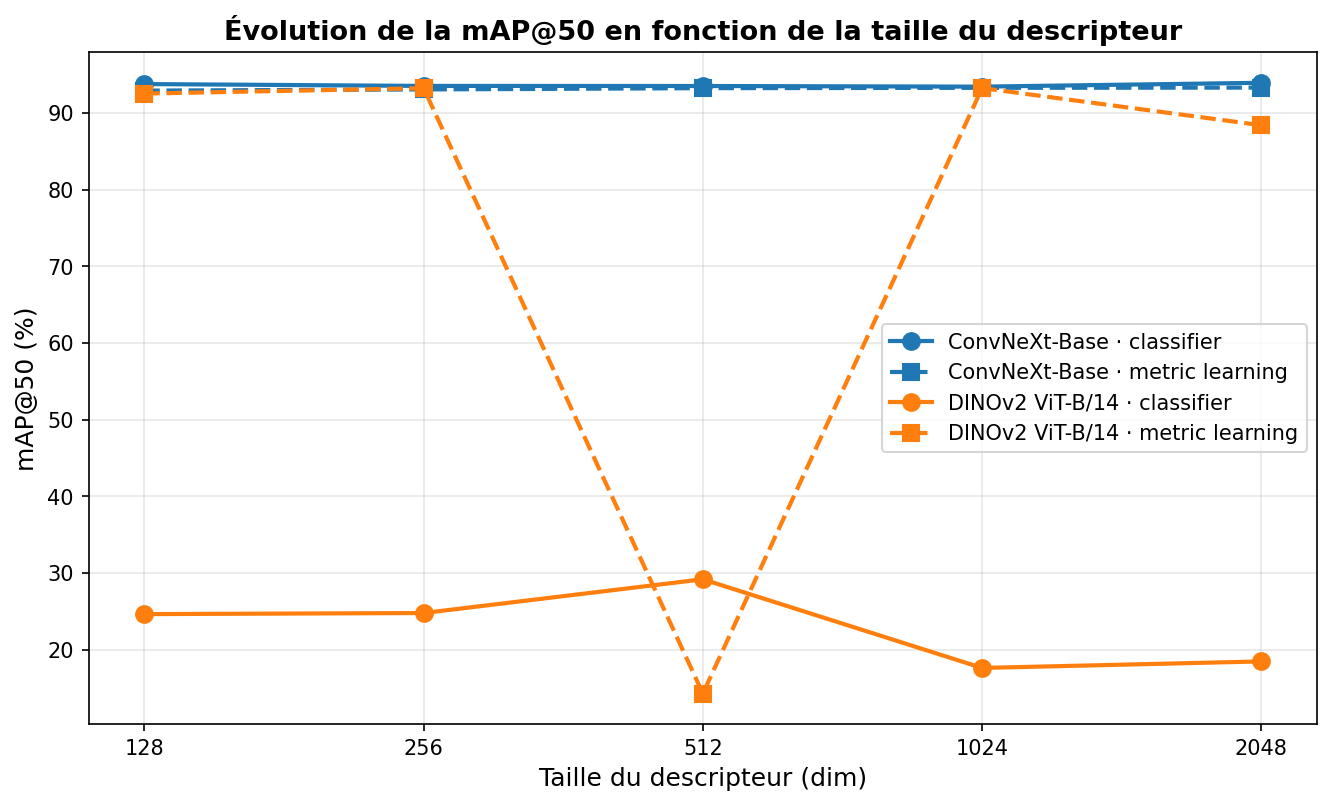
\includegraphics[width=\linewidth]{map50_vs_dim.png}
        \caption{$\text{mAP}@50$.}
        \label{fig:map50}
    \end{subfigure}
    \hfill
    \begin{subfigure}[b]{0.49\textwidth}
        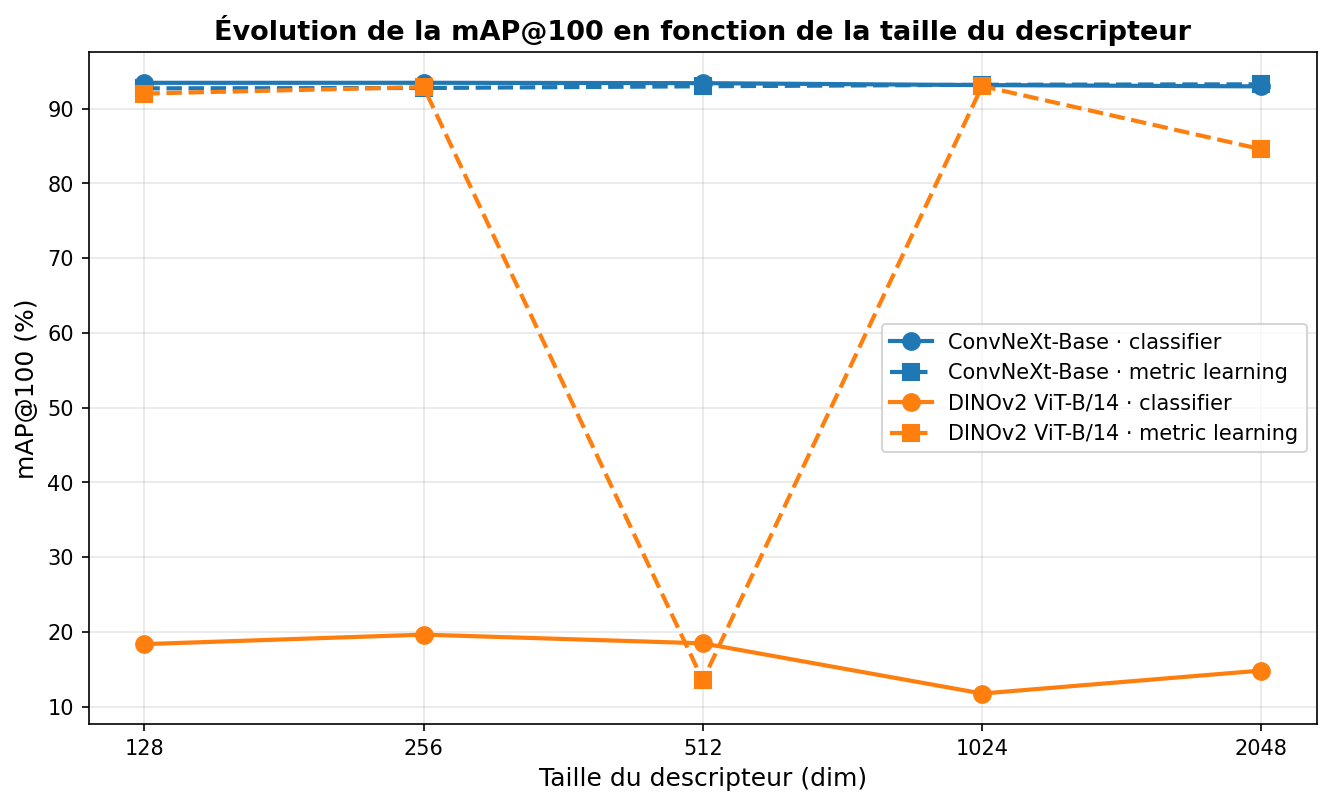
\includegraphics[width=\linewidth]{map100_vs_dim.png}
        \caption{$\text{mAP}@100$.}
        \label{fig:map100}
    \end{subfigure}
    \caption{Évolution de la $\text{mAP}$ en fonction de la dimension
    d'embedding pour les quatre configurations
    $\{\text{ConvNeXt}, \text{DINOv2}\} \times \{\text{classifier},
    \text{metric}\}$.}
    \label{fig:map_vs_dim}
\end{figure}

Trois observations majeures se dégagent~:
\begin{itemize}
    \item \textbf{Saut de performance descripteurs classiques
    $\rightarrow$ profonds}~: on passe de $\sim 5\%$ de $\text{mAP}@50$
    à $\sim 94\%$, soit près de \emph{deux ordres de grandeur}. La
    classification fine marque/modèle exige des représentations
    sémantiques que les descripteurs bas-niveau ne peuvent pas fournir.

    \item \textbf{ConvNeXt vs DINOv2}~: en mode \textit{classifier},
    DINOv2 s'effondre ($\le 30\%$ de $\text{mAP}@50$). L'explication
    tient à la nature self-supervisée du pré-entraînement DINOv2~: les
    \textit{features} sont organisées par similarité visuelle
    \emph{générique} et le \textit{fine-tuning} via une simple
    \texttt{CrossEntropy} sur $96$ classes ne suffit pas à les
    restructurer. À l'inverse, en mode \textit{metric learning}, la perte
    \textit{ArcFace} \emph{réorganise} explicitement l'espace latent et
    permet à DINOv2 de rejoindre ConvNeXt ($93.27\%$ vs $93.96\%$).
    Concrètement, le \textit{metric learning} est \emph{nécessaire} pour
    le ViT et \emph{indifférent} pour le CNN.

    \item \textbf{Robustesse à la réduction de dimension}~: pour
    ConvNeXt, le $\text{mAP}@50$ varie de moins de $1$ point entre
    $d=128$ ($93.80\%$) et $d=2048$ ($93.96\%$), ce qui ouvre la voie à
    une compression $\times 16$ avec perte négligeable - point crucial
    pour le déploiement web (Section~\ref{sec:part3}). DINOv2 metric est
    plus capricieux~: la version $d=512$ s'effondre
    ($\text{mAP}@50 = 14.3\%$) probablement à cause d'une initialisation
    défavorable lors d'un seed unique d'entraînement, alors que les
    voisines $d=256$ et $d=1024$ sont stables au-dessus de $93\%$.
\end{itemize}

\paragraph{Détail par requête.}
La Table~\ref{tab:per_query} reporte les scores du meilleur modèle global
(\textit{ConvNeXt-Base classifier}, $d=2048$) pour chacune des $15$
requêtes. La performance est très homogène ($\text{AP}@50 \ge 96\%$ pour
$14$ requêtes sur $15$), à l'exception remarquable de la requête $R_9$
(\textit{Opel zafiralife}) qui chute à $\text{AP}@50 = 33.3\%$. Cette
dégradation localisée est imputable à la sous-représentation et à
l'apparence atypique du modèle dans le corpus (silhouette de monospace
plus proche d'un Opel Vivaro fourgon que des autres berlines de la
classe). Hors $R_9$, le $\text{mAP}@50$ remonterait à $99.0\%$.

\begin{table}[H]
\centering
\small
\begin{tabular}{lcccccc}
\toprule
Requête & $R@50$ & $R@100$ & $P@50$ & $P@100$ & $AP@50$ & $AP@100$ \\
\midrule
$R_1$  (BMW X3)            & $0.31$ & $0.61$ & $1.00$ & $0.99$ & $1.000$ & $1.000$ \\
$R_2$  (BMW S\'erie 3)     & $0.51$ & $0.70$ & $1.00$ & $0.69$ & $1.000$ & $0.976$ \\
$R_3$  (BMW i8)            & $0.36$ & $0.69$ & $1.00$ & $0.95$ & $1.000$ & $0.997$ \\
$R_4$  (VW Touareg)        & $0.51$ & $0.80$ & $1.00$ & $0.79$ & $1.000$ & $0.990$ \\
$R_5$  (VW Polo)           & $0.51$ & $0.82$ & $1.00$ & $0.81$ & $1.000$ & $0.984$ \\
$R_6$  (VW T-Roc)          & $0.51$ & $0.93$ & $1.00$ & $0.92$ & $1.000$ & $0.995$ \\
$R_7$  (Opel Vivaro)       & $0.49$ & $0.95$ & $0.98$ & $0.94$ & $0.961$ & $0.972$ \\
$R_8$  (Opel Insignia)     & $0.48$ & $0.77$ & $0.96$ & $0.76$ & $0.998$ & $0.966$ \\
$R_9$  (Opel Zafira)       & $0.01$ & $0.07$ & $0.02$ & $0.07$ & $\mathbf{0.333}$ & $\mathbf{0.093}$ \\
$R_{10}$ (Hyundai Nexo)    & $0.51$ & $0.65$ & $1.00$ & $0.64$ & $1.000$ & $0.993$ \\
$R_{11}$ (Hyundai i10)     & $0.34$ & $0.68$ & $1.00$ & $1.00$ & $1.000$ & $1.000$ \\
$R_{12}$ (Hyundai i30)     & $0.51$ & $0.85$ & $1.00$ & $0.84$ & $1.000$ & $0.985$ \\
$R_{13}$ (Ford Puma)       & $0.36$ & $0.72$ & $1.00$ & $1.00$ & $1.000$ & $1.000$ \\
$R_{14}$ (Ford Explorer)   & $0.47$ & $0.92$ & $1.00$ & $0.98$ & $1.000$ & $1.000$ \\
$R_{15}$ (Ford Focus)      & $0.49$ & $0.74$ & $0.98$ & $0.73$ & $0.997$ & $0.990$ \\
\midrule
\textbf{Moyenne (mAP)}    &        &        &        &        & $\mathbf{0.953}$ & $\mathbf{0.929}$ \\
\bottomrule
\end{tabular}
\caption{Table~4 - Métriques par requête pour le meilleur modèle global
(ConvNeXt-Base, mode classifier, $d=2048$).}
\label{tab:per_query}
\end{table}

\subsection{Discussion et choix retenu pour le moteur final}
\label{subsec:discussion_part1}

\paragraph{Choix des trois meilleurs descripteurs.}
Aucun descripteur ne domine simultanément sur tous les critères.
\textit{ConvNeXt classifier} maximise la précision dans le top-50
($\text{mAP}@50 = 93.96\%$), tandis que \textit{ConvNeXt metric} et
\textit{DINOv2 metric} sont marginalement supérieurs au-delà du top-50,
indiquant un classement plus stable en queue. À taille de descripteur
égale ($d=2048$, $78$~MB), le mode \textit{metric} est aussi le plus
rapide à la recherche et bénéficie d'un meilleur \textit{mR-Precision}
($0.86$ vs $0.79$ pour ConvNeXt). Le podium retenu pour la Table~3
est donc~:
\begin{enumerate}
    \item \textbf{ConvNeXt-Base classifier ($d=2048$)} -- meilleur
    $\text{mAP}@50$ ($93.96\%$). \emph{Descripteur CNN}.
    \item \textbf{ConvNeXt-Base metric ($d=2048$)} -- meilleur
    \textit{mR-Precision} parmi les CNN, recherche rapide. \emph{Descripteur CNN}.
    \item \textbf{DINOv2 ViT-B/14 metric ($d=1024$)} -- meilleur
    descripteur de la famille \emph{Vision Transformer}, à empreinte
    mémoire moitié moindre. \emph{Descripteur ViT}.
\end{enumerate}
Cette sélection satisfait la \textbf{Note~1} de l'énoncé qui exige
\emph{au moins deux descripteurs profonds dont un CNN et un ViT parmi
les trois meilleurs}. Dans le moteur déployé en
Section~\ref{sec:part3}, ces trois descripteurs sont sélectionnables
par l'utilisateur, complétés par les descripteurs classiques
(HOG, SIFT-BoVW, ORB-BoVW) à des fins comparatives et pédagogiques.

\paragraph{Apport de la fusion multi-descripteurs.}
La fusion RRF (Eq.~\eqref{eq:rrf}) prend tout son sens lorsque l'on
combine un descripteur classique (sensible aux contours, robuste aux
variations sémantiques fines) et un descripteur profond (sémantiquement
riche mais potentiellement biaisé par les corrélations
d'\textit{ImageNet}). En pratique, sur la base \textit{Cars}, l'écart de
performance entre descripteurs profonds et classiques est tel que la
fusion bénéficie peu au modèle profond seul~; elle reste néanmoins
pertinente pour comparer empiriquement les descripteurs et pour
illustrer la modularité du moteur dans l'interface web.

\paragraph{Réduction de dimension.}
La quasi-platitude de la courbe $\text{mAP}@50(d)$ pour ConvNeXt
(Fig.~\ref{fig:map50}) suggère qu'une représentation de seulement
$128$ flottants ($\sim 4.9$~MB pour la galerie complète) suffit à
capturer l'essentiel de l'information de classe. Cette propriété est
exploitée en Section~\ref{sec:part3} pour réduire l'empreinte mémoire du
service hébergé. Pour DINOv2, la non-monotonie observée à $d=512$
metric appelle à plus de prudence~: en pratique, $d=256$ ou $d=1024$
constituent les choix sûrs.

\paragraph{Limites.}
Les performances rapportées sont obtenues avec une galerie qui contient
le \textit{set} d'entraînement~; bien que les requêtes en aient été
exclues, certaines images très proches (mêmes véhicules sous
différents angles) peuvent figurer dans la galerie d'entraînement. Une
évaluation \textit{val-only} (cellule de contrôle du notebook) confirme
néanmoins que la chute reste limitée à quelques points de $\text{mAP}$,
ce qui valide la robustesse des descripteurs profonds appris.

\newpage
%% Marie
\section{Moteur de recherche multi modal}
\label{sec:part2}


\newpage
\section{Hébergement de ressources cloud}
\label{sec:part3}

%% Marie
\subsection{Interface Web}

%% Flavio
\subsection{Lien entre les modèles et l'interface}
\label{subsec:link_models_ui}

\paragraph{Architecture en trois couches.}
L'application suit une architecture en trois couches strictement séparées
afin de garantir la modularité et de simplifier le déploiement~:
\begin{enumerate}
    \item Une couche \textbf{front-end} statique (HTML, CSS, JavaScript)
    située dans le dossier \texttt{Site\_Internet/}~;
    \item Une couche \textbf{back-end} Flask (\texttt{app.py}) qui
    expose une API REST et qui sert également les fichiers statiques du
    front~;
    \item Une couche \textbf{moteur de recherche} (\texttt{src/part1\_unimodal/}
    et \texttt{src/part2\_multimodal/}) qui encapsule la logique
    d'extraction de descripteurs et de recherche par plus proches
    voisins. Cette couche est totalement agnostique du protocole HTTP
    et peut être réutilisée hors ligne (notebooks, scripts).
\end{enumerate}

\paragraph{Séparation indexation hors-ligne / requête en ligne.}
Comme le suggère l'énoncé (\textit{« the indexing phase should not be
hosted on the deployment resource itself »}), nous distinguons deux
phases~:
\begin{itemize}
    \item \textbf{Hors-ligne}, sur une station équipée d'un GPU~: les
    descripteurs de la galerie sont calculés une fois pour toutes par
    \texttt{extract\_classical.py} (HOG, BoVW pour SIFT et ORB), par les
    notebooks d'entraînement Deep-Learning
    (\texttt{01\_descriptor\_tests\_DeepLearning}) et par
    \texttt{extract\_clip.py} (embeddings CLIP de Flickr8k). Tous ces
    artefacts sont sérialisés dans \texttt{results/features/} sous
    forme de tableaux NumPy et de fichiers JSON.

    \item \textbf{En ligne}, sur le serveur de déploiement~: seul le
    descripteur de la \emph{requête} doit être calculé à la volée, puis
    confronté aux galeries pré-indexées. Cette asymétrie est cruciale~:
    elle permet de tenir des temps de réponse de l'ordre du dixième de
    seconde même sans GPU.
\end{itemize}

\paragraph{API REST exposée.}
Le back-end Flask déclare un nombre minimal d'endpoints, résumés dans la
Table~\ref{tab:api}. La séparation \texttt{/api/search} (unimodal) /
\texttt{/api/search\_multimodal} (texte-image CLIP) reflète directement
les Parties~I et II du projet.

\begin{table}[H]
\centering
\small
\renewcommand{\arraystretch}{1.15}
\begin{tabular}{>{\ttfamily}l>{\ttfamily}cl}
\toprule
\textnormal{Méthode} & \textnormal{Chemin} & \textnormal{Rôle} \\
\midrule
GET  & /api/images            & Liste des fichiers de la galerie \textit{Cars} (autocomplétion) \\
GET  & /cars\_dataset/<name>  & Sert une image du corpus Cars \\
GET  & /flickr\_dataset/<name>& Sert une image du corpus Flickr8k \\
POST & /api/search            & Recherche unimodale (descripteurs Cars) \\
POST & /api/search\_multimodal& Recherche multimodale CLIP (texte ou image) \\
GET  & /api/projection\_3d    & Projection UMAP 3D d'un descripteur (visualisation) \\
\bottomrule
\end{tabular}
\caption{Points d'entrée HTTP exposés par \texttt{app.py}.}
\label{tab:api}
\end{table}

\paragraph{Cycle de vie d'une requête unimodale.}
Lorsque l'utilisateur soumet une recherche depuis \texttt{index2.html},
le frontend envoie une requête \texttt{POST /api/search} contenant, soit
le nom d'un fichier déjà présent dans la galerie (transmis en JSON),
soit une image téléversée (encodée en \texttt{multipart/form-data}),
accompagnée des paramètres \texttt{descriptors[]}, \texttt{metric} et
\texttt{top\_k}. Le handler Flask délègue ensuite à l'une des deux
fonctions du module \texttt{part1\_unimodal.search}~:
\begin{itemize}
    \item \texttt{search()}~: l'image est déjà connue, son vecteur a été
    pré-calculé. La fonction se contente de récupérer le vecteur, de
    calculer les distances aux $N=10\,000$ vecteurs de la galerie et de
    renvoyer les $k$ meilleurs.
    \item \texttt{search\_uploaded()}~: l'image est inédite. Le module
    \texttt{extractors} est sollicité pour calculer le descripteur à la
    volée (HOG via \textit{scikit-image}, BoVW via le \textit{KMeans}
    sérialisé sur disque, embeddings DL via les checkpoints \texttt{.pth}
    chargés en GPU/CPU à la première requête).
\end{itemize}
Dans les deux cas, la réponse JSON renvoie une liste
\texttt{results = [\{filename, score\}, \dots]} accompagnée d'un objet
\texttt{pr\_curve} contenant les vecteurs \emph{recall}, \emph{precision}
et la valeur d'\textit{Average Precision} pour la requête. Le front-end
trace alors la courbe avec \textit{Plotly} et affiche les vignettes
récupérées via \texttt{/cars\_dataset/<name>}.

\paragraph{Cache mémoire et chargement paresseux.}
Pour absorber le coût de chargement des modèles profonds
($\approx 350$~MB pour ConvNeXt et $90$~MB pour DINOv2), chaque module
maintient un dictionnaire \texttt{\_cache} ou \texttt{\_state} chargé
\emph{à la première requête} et conservé en mémoire pour toute la durée
de vie du processus~:
\begin{itemize}
    \item \texttt{part1\_unimodal.extractors} mémorise les modèles
    \textit{torch} et leurs transformations associées, ainsi que les
    vocabulaires BoVW de SIFT/ORB~;
    \item \texttt{part1\_unimodal.search} cache les galeries
    \texttt{.npy} dès leur premier chargement~;
    \item \texttt{part2\_multimodal.faiss\_index} construit l'index
    FAISS~\texttt{IndexFlatIP} \emph{une seule fois} (la première
    requête multimodale paie le coût d'initialisation, les suivantes
    sont quasi-instantanées)~;
    \item \texttt{part2\_multimodal.clip\_encoder} ne charge le modèle
    \texttt{openai/clip-vit-base-patch32} qu'au premier appel.
\end{itemize}
Cette stratégie de \textit{lazy loading} permet à l'application de
démarrer en quelques secondes (contre plusieurs dizaines de secondes
si tous les modèles étaient chargés à l'import) et limite l'empreinte
mémoire aux modules réellement sollicités par l'utilisateur.

\paragraph{Réduction de dimension côté serveur.}
Les courbes de la Section~\ref{subsec:results_part1}
(Fig.~\ref{fig:map_vs_dim}) montrent qu'un descripteur de dimension
$d=128$ pour ConvNeXt préserve l'essentiel de la performance. Pour
réduire l'empreinte hébergée, deux approches sont possibles : soit
réentraîner un modèle à dimension cible directement, ce que nous avons
fait pour ConvNeXt et DINOv2 lors de la grille
$d \in \{128,256,512,1024,2048\}$~; soit appliquer une projection
linéaire (PCA) sur les descripteurs déjà calculés. La première solution
est privilégiée dans le moteur final car elle ne demande qu'un échange
de checkpoint, sans logique additionnelle dans le code de recherche.

\subsection{Hébergement sur un serveur}
\label{subsec:hosting}

\paragraph{Conteneurisation Docker.}
L'application est entièrement conteneurisée via le \texttt{Dockerfile}
présent à la racine du dépôt. L'image est construite à partir de
\texttt{python:3.11-slim} pour minimiser la taille~; seules trois
dépendances système sont installées via \texttt{apt-get} (\texttt{git}
pour récupérer le paquet \textit{CLIP} d'OpenAI, \texttt{libgl1} et
\texttt{libglib2.0-0} pour les bindings OpenCV). Les dépendances Python
sont résolues par \texttt{uv}, gestionnaire de paquets compatible
\texttt{pip} qui synchronise l'environnement système à partir de
\texttt{pyproject.toml} et du \textit{lock file} \texttt{uv.lock}~:
\begin{verbatim}
RUN pip install --no-cache-dir uv \
 && uv pip install --system -r pyproject.toml
\end{verbatim}
Une fois les dépendances installées, le code source (\texttt{app.py},
\texttt{src/}, \texttt{Site\_Internet/}) ainsi que les artefacts
pré-calculés (\texttt{models/}, \texttt{results/}, \texttt{data/}) sont
copiés dans l'image. L'image expose le port \textbf{5000}
(\texttt{EXPOSE 5000}) et démarre Flask via la commande
\texttt{python app.py}, qui appelle
\texttt{app.run(host=\textquotesingle 0.0.0.0\textquotesingle{}, port=5000, debug=False)}
afin d'écouter sur toutes les interfaces.

\paragraph{Optimisations de l'image.}
Plusieurs choix réduisent significativement la taille finale du
conteneur~:
\begin{itemize}
    \item \textbf{Slim base}~: \texttt{python:3.11-slim} pèse $\sim 45$~MB
    contre $\sim 350$~MB pour l'image \texttt{python:3.11} complète~;
    \item \textbf{Variables d'environnement}~:
    \texttt{PYTHONDONTWRITEBYTECODE=1} évite la création de fichiers
    \texttt{.pyc}, \texttt{PIP\_NO\_CACHE\_DIR=1} supprime le cache
    \texttt{pip}, \texttt{PYTHONUNBUFFERED=1} garantit que les logs
    Flask remontent en temps réel dans le journal Docker~;
    \item \textbf{\texttt{.dockerignore}}~: exclut \texttt{.git},
    \texttt{.venv}, \texttt{notebooks/}, \texttt{docs/}, et tous les
    fichiers \texttt{.md} sauf le \texttt{README.md}, ce qui empêche
    l'inclusion de l'historique git, du PDF du rapport ou des
    \textit{checkpoints} de notebooks dans le contexte de \textit{build}.
\end{itemize}

\paragraph{Considérations de sécurité.}
Conformément au point~8 de l'énoncé, plusieurs garde-fous ont été mis en
place~:
\begin{itemize}
    \item \textbf{Mode debug désactivé}~: \texttt{debug=False} en
    production prévient l'exposition du \textit{Werkzeug debugger} (qui
    autorise l'exécution arbitraire de code via la console)~;

    \item \textbf{Validation des entrées}~: tout paramètre numérique
    (\texttt{top\_k}) est explicitement converti en \texttt{int} avec
    capture de l'exception et code HTTP $400$~; les noms de descripteurs
    sont validés contre la \textit{whitelist}
    \texttt{DESCRIPTOR\_TAGS} dans \texttt{search.py}~;

    \item \textbf{Protection contre le \textit{path traversal}}~: les
    routes \texttt{/cars\_dataset/<name>} et
    \texttt{/flickr\_dataset/<name>} utilisent \texttt{send\_from\_directory}
    qui résout les chemins relativement à un dossier ancré et rejette
    tout chemin hors arborescence (\texttt{../..} etc.)~;

    \item \textbf{Pas de secrets dans l'image}~: la clé
    \texttt{WANDB\_API\_KEY} (utilisée uniquement à l'entraînement)
    n'est jamais lue par \texttt{app.py} et le fichier
    \texttt{.env} est exclu du conteneur via \texttt{.dockerignore}.

    \item \textbf{Surface d'attaque réduite}~: l'image n'expose qu'un
    seul port et n'embarque ni \textit{shell} interactif, ni outil
    réseau (\texttt{curl}, \texttt{wget}, \texttt{netcat} ne sont pas
    installés sur la base \textit{slim}).
\end{itemize}
Une analyse complémentaire (\textit{rate limiting}, en-têtes HTTPS via
un reverse-proxy, cookies de session, page de connexion) reste à
l'étude pour une mise en production publique. Pour le périmètre de ce
projet, l'application est destinée à une démonstration ponctuelle et la
liste précédente couvre les vecteurs les plus critiques.

\paragraph{Déploiement.}
Le déploiement se fait en deux commandes une fois Docker installé sur
le serveur cible~:
\begin{verbatim}
docker build -t mir-app .
docker run -d -p 80:5000 --name mir mir-app
\end{verbatim}
Le mappage \texttt{-p 80:5000} expose l'application sur le port HTTP
standard. L'image construite ($\sim 4$~GB, dominée par les
\textit{checkpoints} \texttt{.pth} de la grille de descripteurs et par
le corpus \textit{Cars}/\textit{Flickr8k} embarqué) reste compatible
avec un déploiement sur les services gratuits suggérés dans l'énoncé
(Oracle Free Tier, Render, Railway). Pour un déploiement en production
plus exigeant, il serait préférable de découpler les artefacts
volumineux dans un volume persistant ou un \textit{object store}
(par exemple S3) plutôt que de les empaqueter dans l'image.

\newpage
\section{Conclusion}
\label{sec:conclusion}

Ce projet a abouti à la conception, l'implémentation et le déploiement
d'une application complète de recherche multimédia, articulée autour de
trois axes complémentaires.

En \textbf{Partie~I}, le moteur unimodal sur la base \textit{Cars} a
montré que les descripteurs profonds dépassent de près de \emph{deux
ordres de grandeur} les descripteurs classiques (HOG, SIFT-BoVW,
ORB-BoVW) sur la tâche fine de discrimination
\textit{marque + modèle}~: $\text{mAP}@50 \approx 94\%$ pour
\textit{ConvNeXt-Base classifier} contre moins de $5\%$ pour les
meilleurs descripteurs \textit{hand-crafted}. La comparaison
systématique entre paradigmes \textit{classifier} et \textit{metric
learning} a aussi révélé un comportement très différent selon
l'architecture~: ConvNeXt obtient des résultats équivalents dans les
deux modes alors que DINOv2 ne devient compétitif qu'avec une perte
\textit{ArcFace}, ce qui reflète l'origine self-supervisée de son
pré-entraînement. Enfin, l'étude de la grille
$d \in \{128,\dots,2048\}$ a montré une remarquable robustesse à la
réduction de dimension, qui ouvre la voie à des descripteurs très
compacts ($\sim 5$~MB pour la galerie complète) sans perte sensible.

En \textbf{Partie~II}, le moteur multimodal sur \textit{Flickr8K}
exploite l'espace latent partagé de CLIP pour offrir des recherches
\textit{texte $\to$ image} et \textit{image $\to$ image} indexées par
FAISS. La rapidité de la recherche (de l'ordre de la milliseconde par
requête) et la qualité sémantique des résultats valident l'intérêt des
modèles contrastifs pré-entraînés à grande échelle pour la recherche
multimédia, sans coût d'entraînement supplémentaire.

En \textbf{Partie~III}, l'ensemble a été encapsulé dans un service web
Flask conteneurisé. La séparation stricte entre indexation hors-ligne
et inférence en ligne, combinée à un \textit{lazy loading} des modèles,
permet à l'application de répondre en quelques centaines de
millisecondes sans nécessiter de GPU sur le serveur de déploiement.

\paragraph{Perspectives.}
Plusieurs pistes d'amélioration mériteraient d'être explorées au-delà
du cadre de ce projet~:
\begin{itemize}
    \item Remplacer l'index exact \texttt{IndexFlatIP} de FAISS par un
    index approché (\texttt{IVF}, \texttt{HNSW}, \texttt{PQ}) pour
    passer à l'échelle au-delà de quelques dizaines de milliers
    d'images~;

    \item Étendre la fusion multi-descripteurs au-delà du Reciprocal
    Rank Fusion par des approches apprises (\textit{learning-to-rank})
    qui pondéreraient explicitement les contributions de chaque
    descripteur~;

    \item Affiner CLIP par \textit{fine-tuning} contrastif sur
    \textit{Flickr8K} ou comparer plus systématiquement à BLIP/OpenCLIP
    pour quantifier le gain attendu sur ce domaine spécifique~;

    \item Industrialiser le déploiement en externalisant les
    \textit{checkpoints} et le corpus dans un \textit{object store},
    en ajoutant un reverse-proxy HTTPS et une page d'authentification.
\end{itemize}
Ces extensions ne remettent toutefois pas en cause le constat principal
de ce travail~: la combinaison d'un descripteur profond bien choisi,
d'une indexation efficace et d'une interface web légère suffit à
construire un moteur de recherche multimédia performant et déployable.

\newpage
\printbibliography

\end{document}
